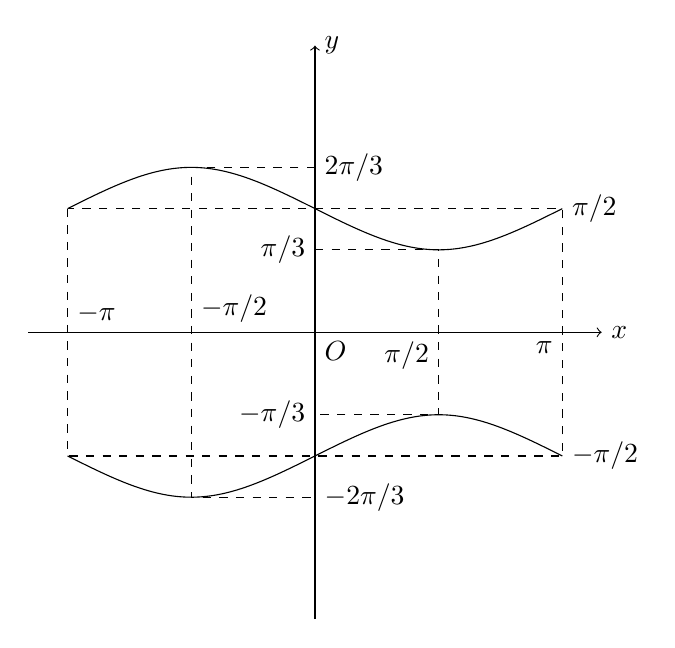
\begin{tikzpicture}[trig format=rad]
    \draw[->] (-pi - 0.5, 0) -- (pi + 0.5, 0) node[right] {\(x\)};
    \draw[->] (0, -pi - 0.5) -- (0, pi + 0.5) node[right] {\(y\)};
    \draw [smooth, samples=200, domain=-pi:pi] plot (\x, {acos(0.5*sin(\x))});
    \draw [smooth, samples=200, domain=-pi:pi] plot (\x, {- acos(0.5*sin(\x))});

    \draw [dashed] (-pi, pi / 2) -- (-pi, -pi / 2) -- (pi, -pi / 2) -- (pi, pi / 2) -- cycle;
    \draw [dashed] (0, pi / 3) -- (pi / 2, pi / 3) -- (pi / 2, -pi / 3) -- (0, -pi / 3);
    \draw [dashed] (0, 2 * pi / 3) -- (-pi / 2, 2 * pi / 3) -- (-pi / 2, -2 * pi / 3) -- (0, -2 * pi / 3);

    \node at (0, 0) [below right] {\(O\)};
    \node at (-pi, 0) [above right] {\(-\pi\)};
    \node at (-pi / 2, 0) [above right] {\(-\pi / 2\)};
    \node at (pi / 2, 0) [below left] {\(\pi / 2\)};
    \node at (pi, 0) [below left] {\(\pi\)};

    \node at (0, -2 * pi / 3) [right] {\(-2\pi / 3\)};
    \node at (pi, -pi / 2) [right] {\(-\pi / 2\)};
    \node at (0, -pi / 3) [left] {\(-\pi / 3\)};
    \node at (0, pi / 3) [left] {\(\pi / 3\)};
    \node at (pi, pi / 2) [right] {\(\pi / 2\)};
    \node at (0, 2 * pi / 3) [right] {\(2\pi / 3\)};
\end{tikzpicture}